% !TEX root = ../thesis.tex
\chapter{Results and Discussion}
\label{chap:results}

We will first look at the web application results based on the user's feedback, and then we will look into the insights and potential feedback the NLP process could provide the user. We then also look to review the overall process. 

We will compare the web application's results against the comparative judgment, Elo ranking, and the score we created for the tweets on Twitter. With the insights of the NLP for feedback to the user, we will look at what insights got made. Additionally, we will look at if any of the knowledge extracted generated provides any meaningful feedback to the user.



\section{Tweet Ranking Results} 
\label{sec:reaults_ranking}

	\begin{figure}[h]
		\centering
		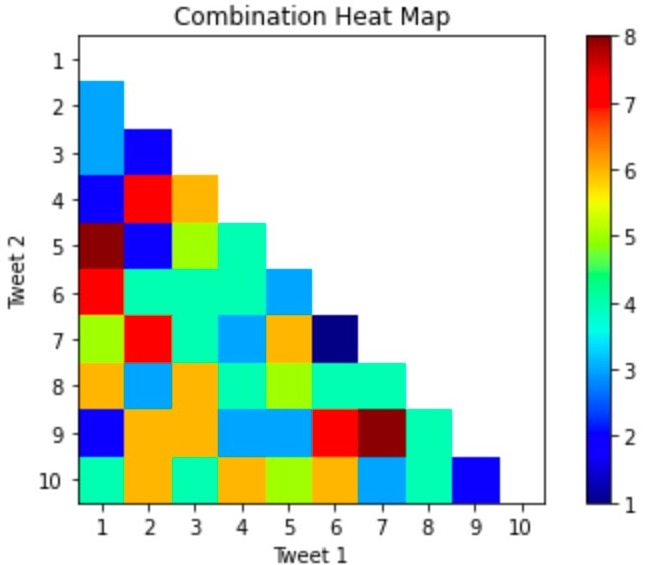
\includegraphics[width=7cm]{combination_heat_map.png}
		\caption{The web applicaitons generated results compared agaist each other.}
		\label{fig:combinations}
		
	\end{figure}
	
	Forty different users take part in the comparison judgement within the web app. Through looking at fig: \ref{fig:combinations} we can see that all combinations got displayed to the users taking part in the comparisons. We can see that tweet one and tweet five appeared the most, while the combination appearing the lowest was tweet six and seven, with one comparison getting presented to the users.
	
	
	
	When we look at winners and losers of the comparisons( see fig: \ref{fig:combination_wins}), we can see that the tweet that won the most between a specific combination was tweet four and two, with tweet four winning six times and tweet two winning only once. Additionally, when we look at the combination that appeared the most, one and five, one came out on top five times, compared to five winning between the two once.
	\begin{figure}[h]
		\centering
		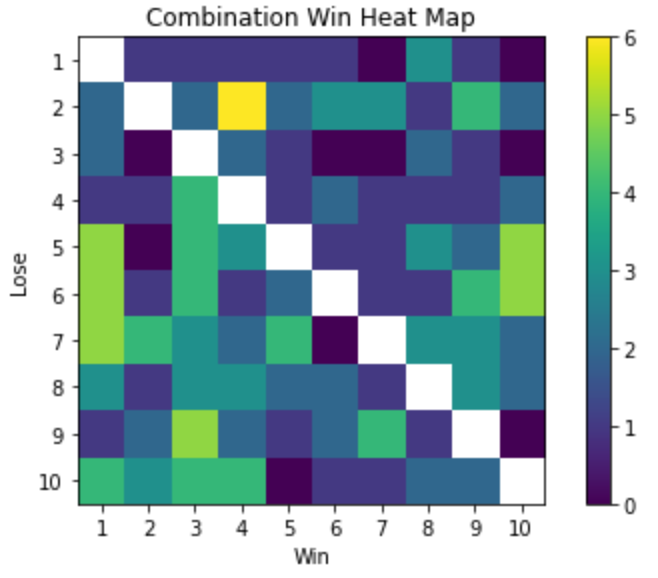
\includegraphics[width=7cm]{combination_win_heat_map.png}
		\caption{A heat map of the amount of times a tweet win or lost}
		\label{fig:combination_wins}
		
	\end{figure}
	
	When we look at the winner heat map (see fig: \ref{fig:combination_wins}), we can see that two, five, six, seven and ten had moments where they didn't win a head-to-head with another tweet. Two, six, seven and ten didn't win against at least two different tweets, while the others were only against one tweet they failed to win.
	
	
	While looking at fig \ref{fig:web_app_results}, we can see that the Elo and comparative judgement ranking generated very similar results. However, as we can see, the tweets coming in 6th, 7th and 8th a slight variation in the results.
	
	\begin{figure}[h]
		\centering
		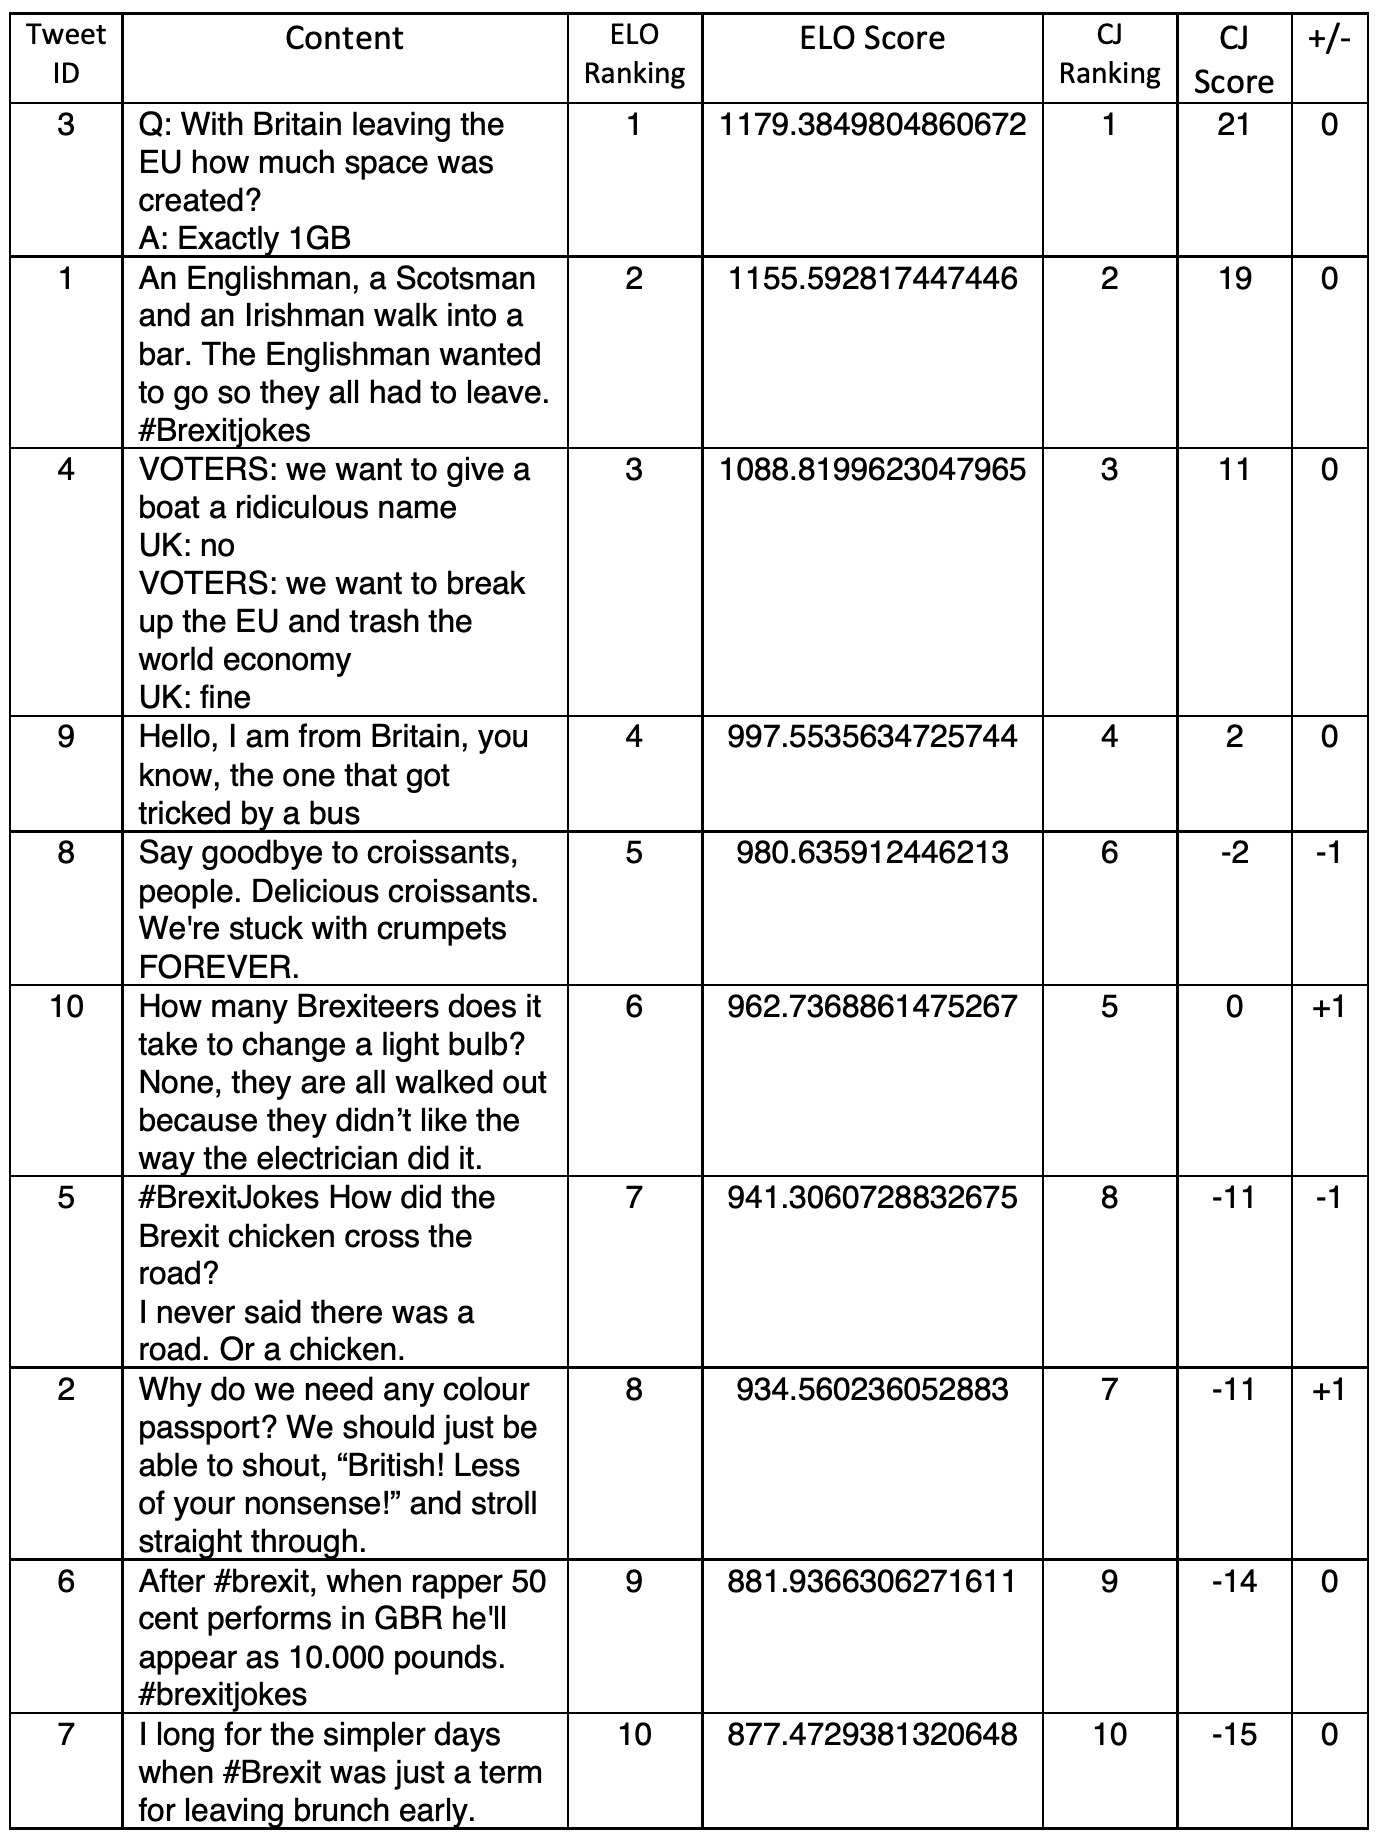
\includegraphics[width=10cm]{web_app_results.png}
		\caption{The web applicaitons generated results compared agaist each other.}
		\label{fig:web_app_results}
		
	\end{figure}

	While we look at the T-rating ranking compared to the Elo ranking (see fig: \ref{fig:twitter_results_comparison}), we can see that the results ranking is very different. The tweet that came first in the T-rankings came fourth in the Elo ranking. At the same time, the tweet that came first in the Elo ranking came eighth in the T-ranking.  Tweets that done worse in the Elo ranking compared to T-ranking had an average difference in the ranked placing of 5 places, while the tweets that had a better Elo ranking compared to the T-ranking ranked an average of 4 places lower. Therefore, 4 of the top 5 tweets in the T-ranking were actually in the bottom five of the Elo ranking. Only tweet ID 4 done one place better with the Elo ranking than it did in the T-ranking. However, two of the top three tweets in the T-ranking were in the bottom three of the Elo ranking and vice versa.

	\begin{figure}[h]
		\centering
		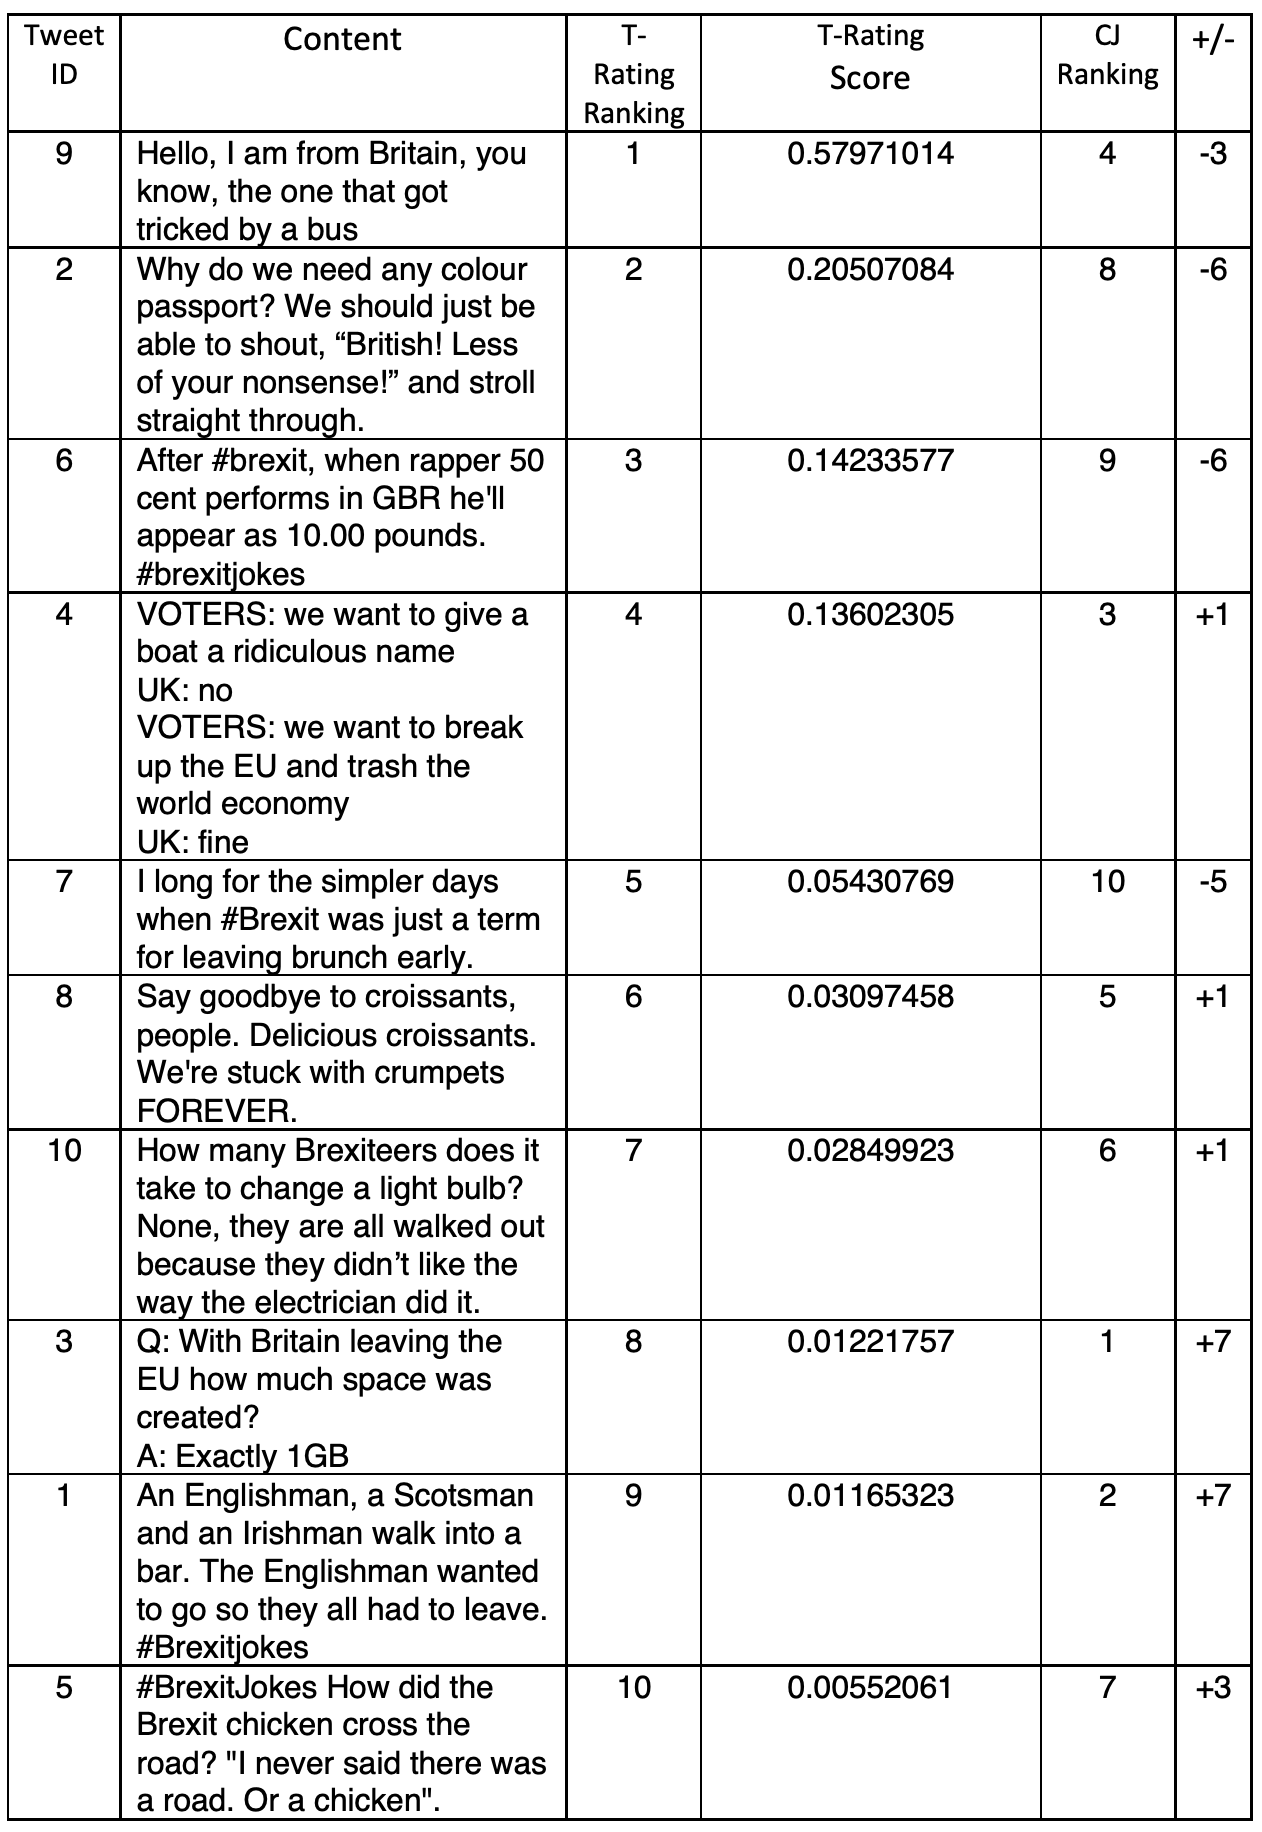
\includegraphics[width=10cm]{twitter_results_comparison.png}
		\caption{The Twitter tweet score ranking comparison against Elo ranking.}
		\label{fig:twitter_results_comparison}
		
	\end{figure}

	Within the forty participants, twenty-two of them left a justification for why they select one tweet over the other. However, the participants' responses were varied in the amount of provided feedback. Some proved a justification for all five combinations. On the other hand, some only left them for a few and not all. The users gave a total of sixty-three explanations to their decisions on which tweet they had chosen.
	
	One user stated, "I just think it is a clever way to put our departure from EU, plus it did make me giggle." The comment was in regards to tweet three beating tweet eight. Tweet three did provide several justifications, a lot of them to do around its tech theme on Brexit. Some of the rationales are "Comp sci wordplay", "everyone loves a tech joke", "Because it's the nerdier option", the "First tweet just lol", and "Actually laughed out loud".
	
	Another tweet, tweet ten beating tweet 8, had the justification for winning as 'because of the wordplay'. So we can see that several tweets had some form of explanation around the lines of good wordplay. Therefore, creating user feedback has not made an excellent source of information to help build feedback. However, it has given some context to why they had made their decisions.


\section{NLP Feedback and Insights}
\label{sec:reaults_NLP}

	The Jupyter notebook was able to conduct the NLP tasks that we required successfully. We presented the user the POS tagging insights of how many POS tags were present in each tweet. We were also able to visualise the POS tagging to reflect the user how the tweet got broken down structure-wise (see fig: \ref{fig:POS_example}).
	
	\begin{figure}[h]
		\centering
		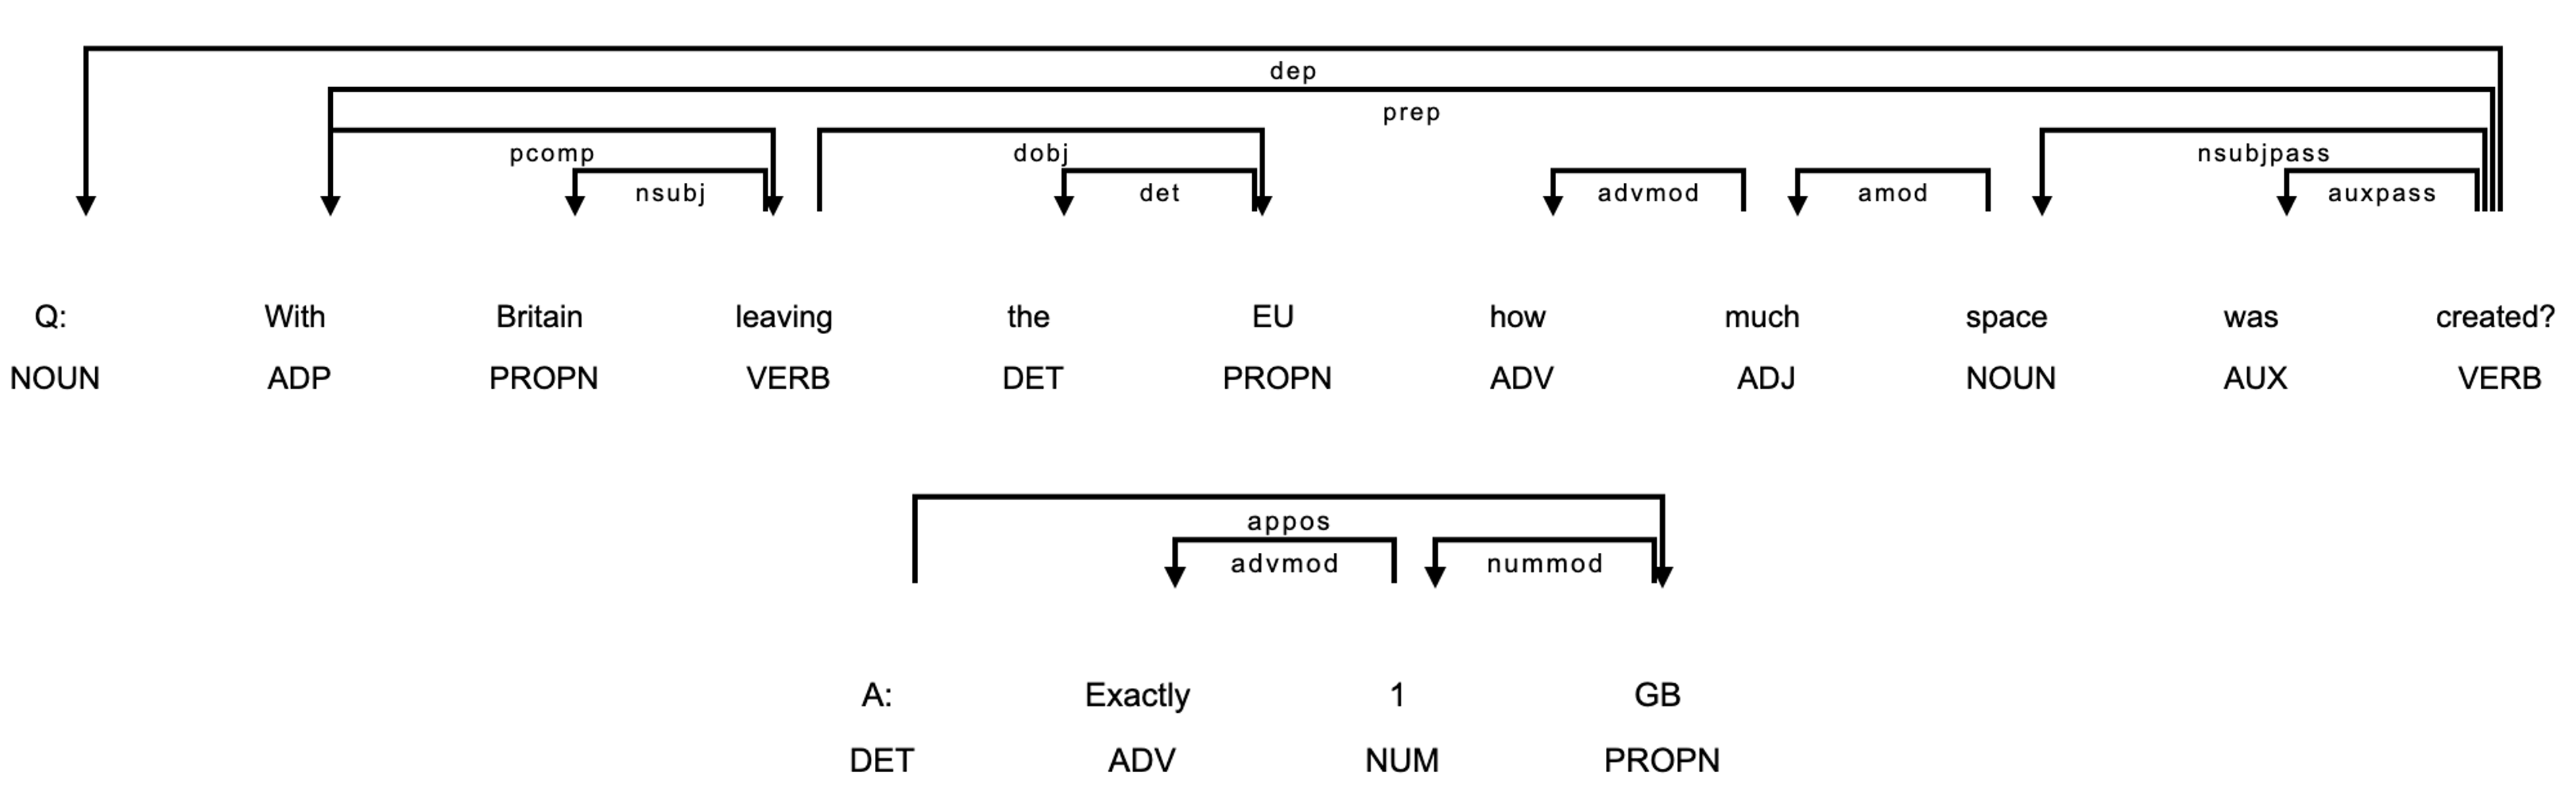
\includegraphics[width=\textwidth]{POS_vis.png}
		\caption{An example of a POS tagging visulaisation.}
		\label{fig:POS_example}
		
	\end{figure}

	We were also able to present to the user the NER that the pre-trained model supplied by spaCy was able to identify. These were presented to the user in text format as well within a visualisation, identifying the NERs within the sentence (see fig: \ref{fig:NER_example}).
	
	\begin{figure}[h]
		\centering
		
\includegraphics[width=\textwidth]{NER_vis.png}
		\caption{An example of a NER tagging visulaisation.}
		\label{fig:NER_example}
		
	\end{figure}

	The notebook was also able to present back to the user the top ten tweets on how similar they were by the whole tweet (see fig: \ref{fig:top_10_sim_doc}) and by NERs (see fig: \ref{fig:top_10_sim_NER}). When looking at the results for the similarity scoring between the NERs, we can see that the most similar tweets are tweet three and tweet 4. These tweets have a similarity score of 0.857896 based on the NER values Britain, EU (Tweet 1) and UK, EU (Tweet 4). The tweets with the least similarity are Tweet 2, British, and Tweet 6, 50, cent, 10.00, pounds, with a similarity score of -0.025753.
	 
	
	\begin{figure}[h]
		\centering
		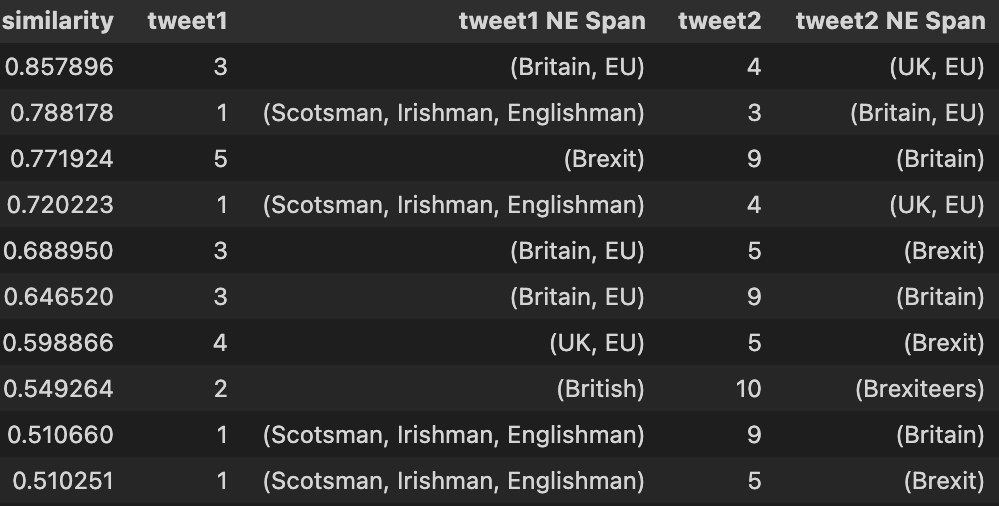
\includegraphics[width=10cm]{top_10_sim_NER.png}
		\caption{A table displaying the top ten similar tweets based on the tweet's NERs.}
		\label{fig:top_10_sim_NER}
		
	\end{figure}

	The results show us, in regards to the whole tweets, that Tweet 5 and Tweet 10 were the most similar with a similarity score of 0.576191. The tweet's contents were '\#BrexitJokes How did the Brexit chicken cross the road? "I never said there was a road. Or a chicken".' (Tweet 5) and 'How many Brexiteers does it take to change a light bulb? None, they are all walked out because they didn't like the way the electrician did it.' (Tweet 10). The tweets with the least similarity are Tweet 4, 'VOTERS: we want to give a boat a ridiculous name UK: no VOTERS: we want to break up the EU and trash the world economy UK: fine', and Tweet 6, 'After \#brexit, when rapper 50 cent performs in GBR he'll appear as 10.00 pounds. \#brexitjokes', with a similarity score of -0.041637.

	\begin{figure}[h]
		\centering
		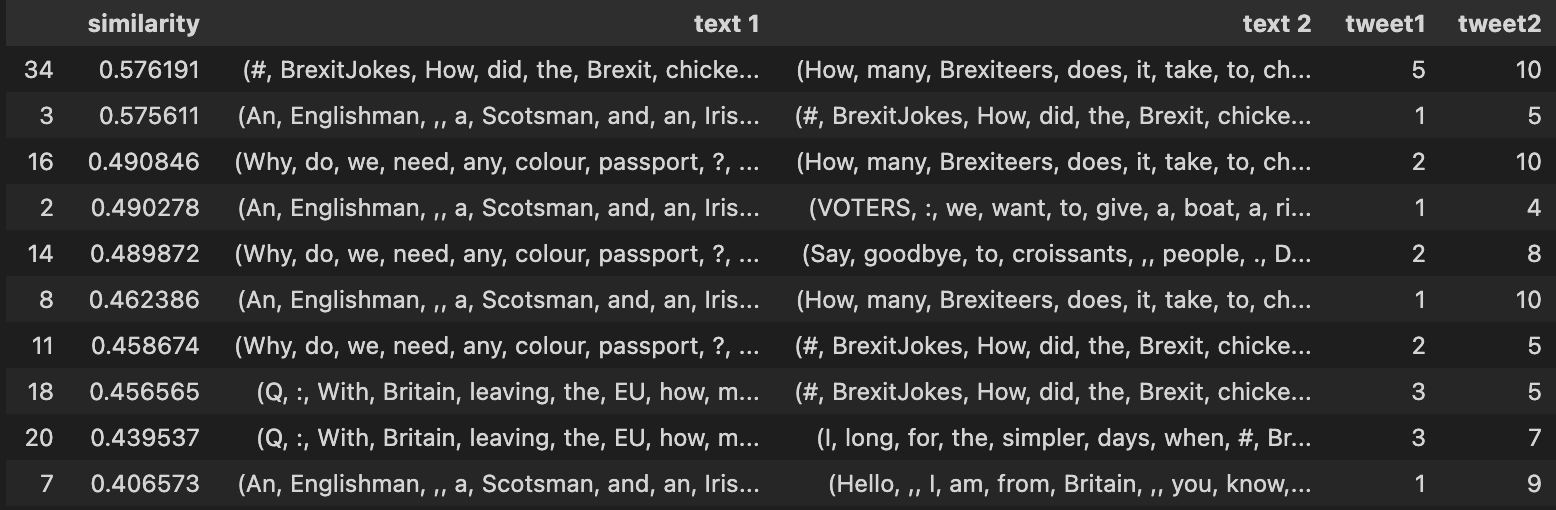
\includegraphics[width=15cm]{top_10_sim_doc.png}
		\caption{A table displaying the top ten similar tweets based on the whole tweet.}
		\label{fig:top_10_sim_doc}
		
	\end{figure}

	The information extraction process identified several interesting aspects from the tweets (see fig: \ref{fig:information_extract}). The results show that six of the tweet's sentiments scoring got classified as positive, and out of those six, five were in the top 5 results. We can't say for certain that having a positive tweet will likely score higher, as the dataset is not big enough to make that kind of claim. However, it does provide some good feedback and insights to the user. The NLP process also provided some excellent extraction of key phrases from the tweets. The only tweet's key phrase that didn't prove any meaningful information was Tweet 7's 'Brexit was'. Considering that these information extraction techniques, NER and key phrases, have not had any additional training, other than what comes out of the box, they have performed well in providing insights and feedback to the user.


	\begin{figure}[h]
		\centering
		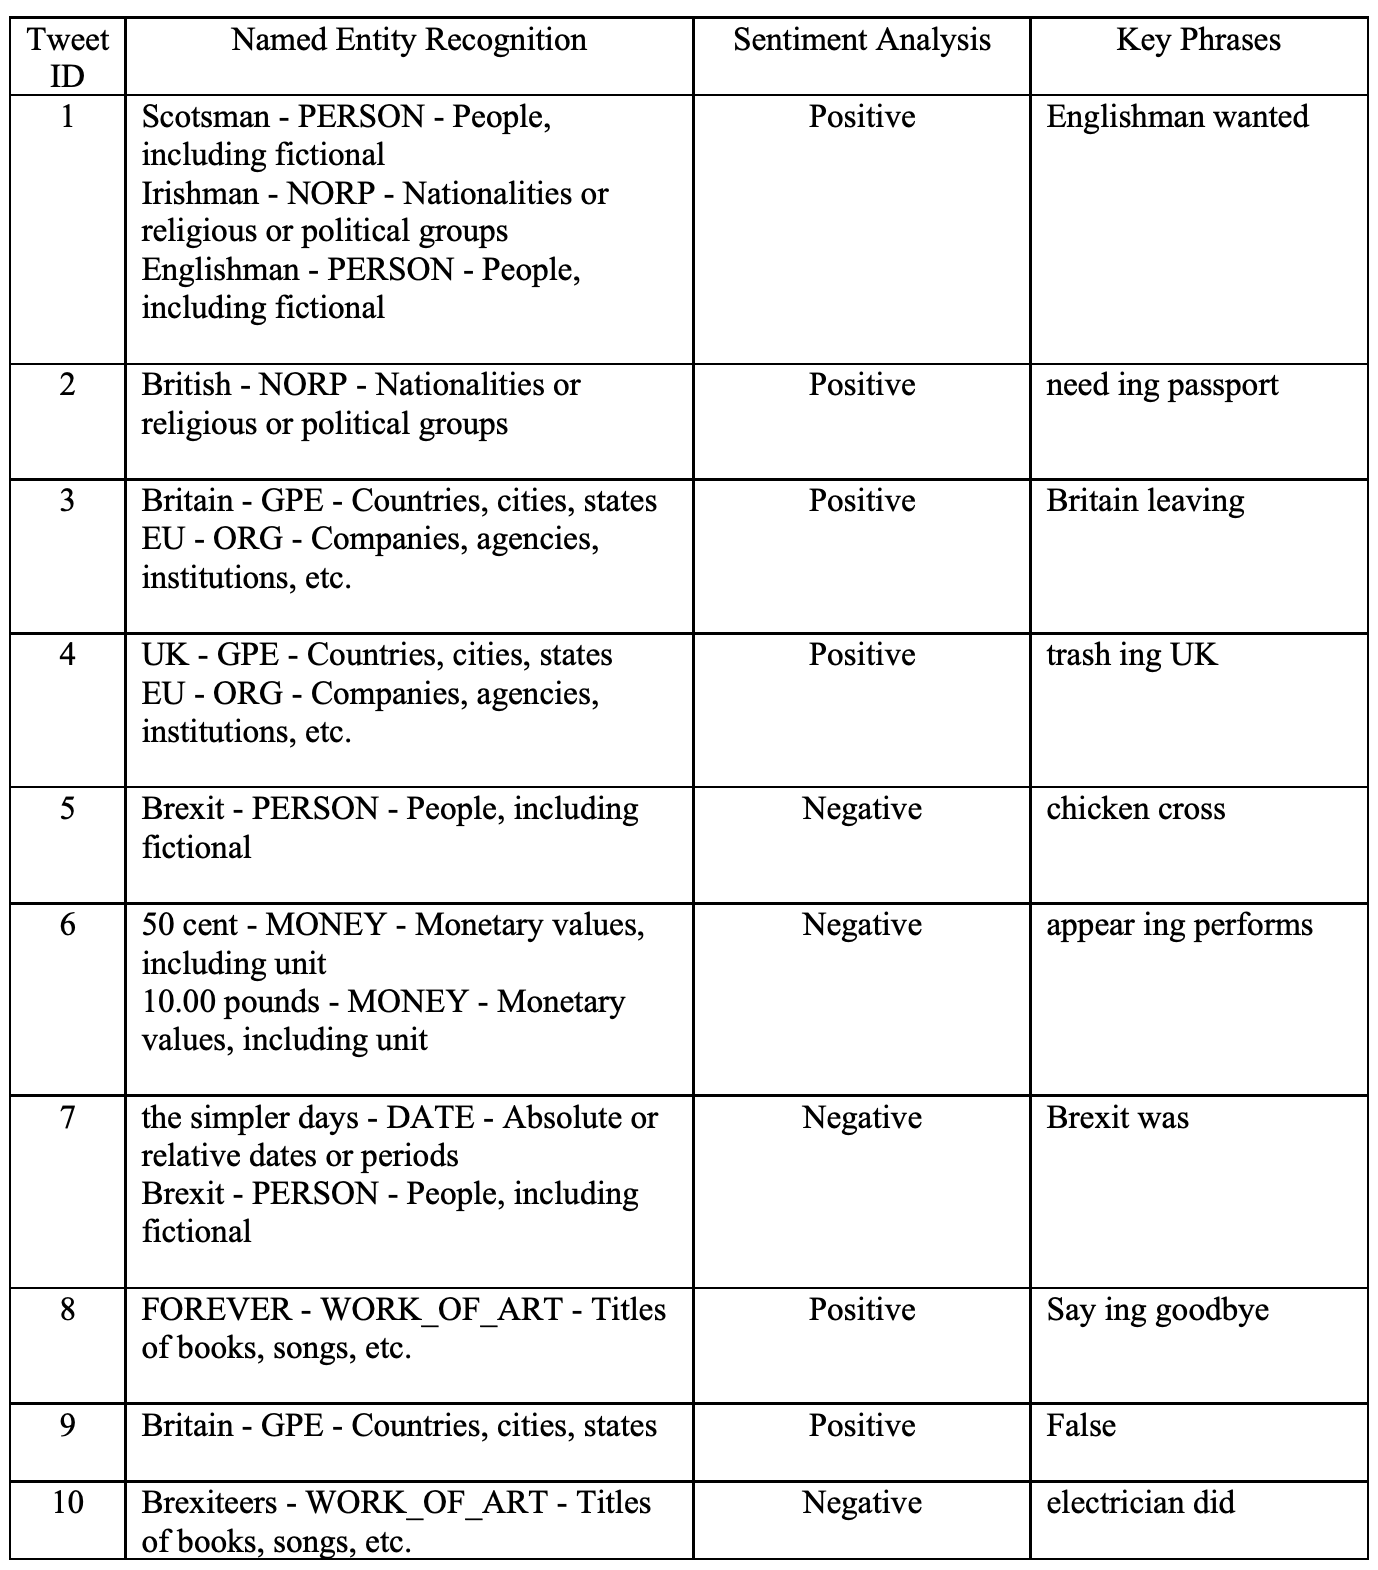
\includegraphics[width=10cm]{information_extract.png}
		\caption{A table displaying the key information extracted from the NER, Sentiment analysis and Key Phrases NLP processes.}
		\label{fig:information_extract}
		
	\end{figure}

	Using the TF-IDF, we extracted the key token features from all of the tweets. The higher the value, the more important that feature is for that tweet (see fig: \ref{fig:feature_extract}). However, this information does not provide much feedback for a user, but it would highly likely be adequate for training some form of ML models.

	\begin{figure}[h]
		\centering
		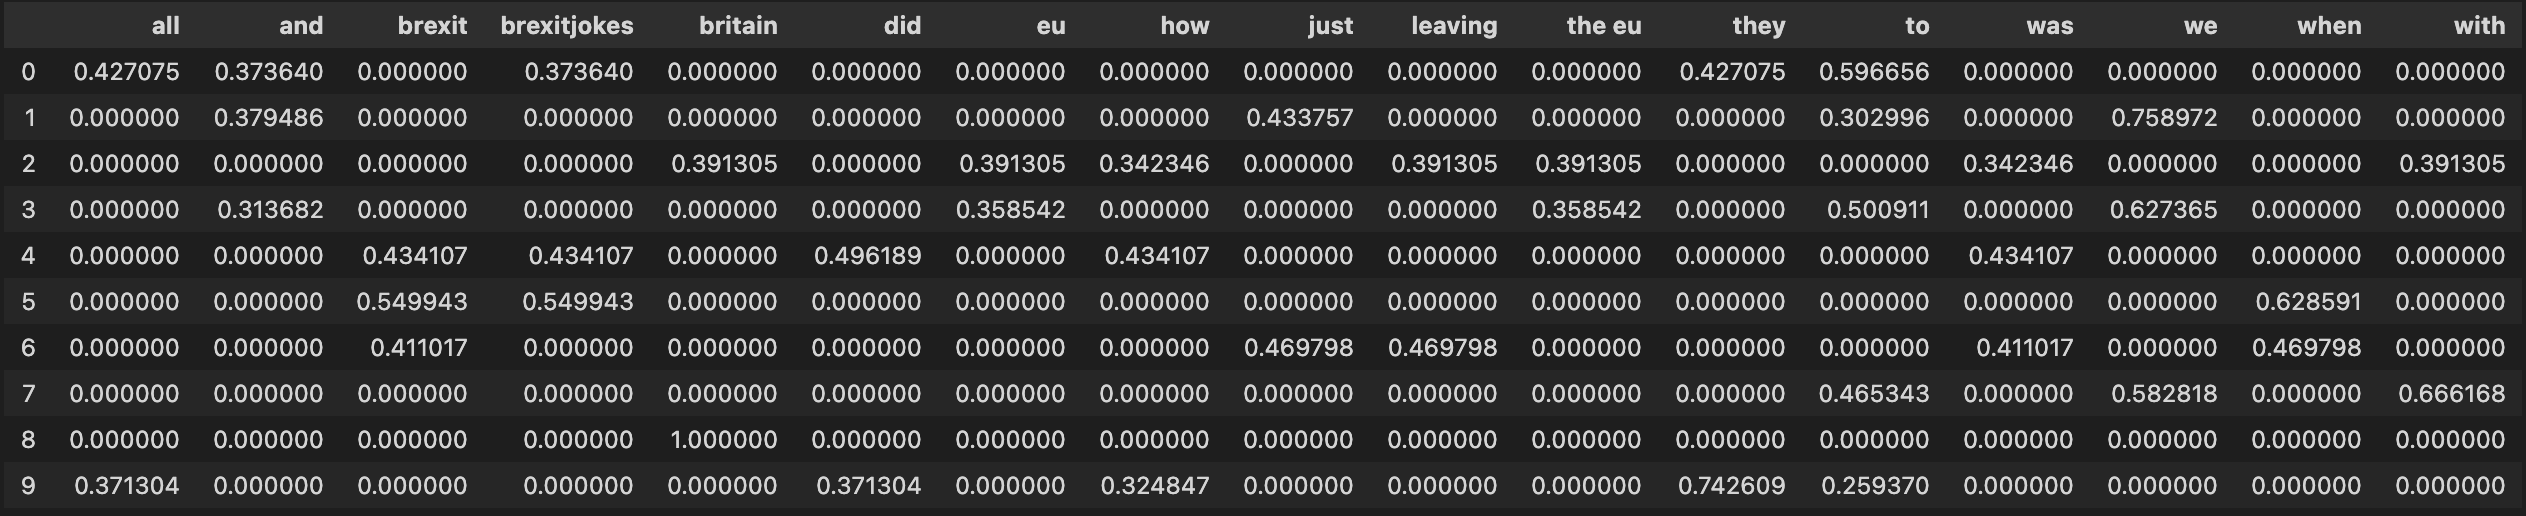
\includegraphics[width=\textwidth]{feat_extra_importance.png}
		\caption{A table showing the key tokens within each tweet and thir importance to that tweet.}
		\label{fig:feature_extract}
		
	\end{figure}

	\textbf{In contrast, the information extraction techniques of blah blah, did not provide any meaningful information. The blah present blah, and the blah presented blah. These techniques have not provided much use currently but could be helpful when scaling up and using a much bigger dataset, like exam papers.}



\section{Overall Results}
\label{sec:reaults_NLP}

	Overall we can suggest that the Elo ranking is a great alternative ranking system to the ACJ. It provides a robust scoring system because the combination process is random, removing any opportunity for Elo's flaws to be taken advantage of. It also provides the ability to try 'what if' calculations with potential comparison outcomes.
	
	On the other hand, the NLP information extraction provided some good information but was too basic to offer any real insights to the user to digest easily. While there is a lot of promise regarding the NLP, more fine-tuning is required to make this feature to provide feedback worthwhile. However, we believe this is a step worth taking with appropriate building blocks that have been put in place to expand upon.

